\documentclass[journal]{IEEEtran}
\usepackage{amsmath,amssymb,amsfonts}
\usepackage{tabularx}
\usepackage[utf8]{inputenc} % allow utf-8 input
\usepackage[T1]{fontenc}    % use 8-bit T1 fonts
\usepackage{url}            % simple URL typesetting
\usepackage{booktabs}       % professional-quality tables
\usepackage{amsfonts}       % blackboard math symbols
\usepackage{nicefrac}       % compact symbols for 1/2, etc.
\usepackage{microtype}      % microtypography
\usepackage{graphicx}
\usepackage{float}
\restylefloat{table}
\usepackage{hyperref}
\usepackage{multicol}
\usepackage{caption}
\usepackage{subcaption}
\usepackage{amsmath}
\usepackage{algorithm}
\usepackage{algpseudocode}
\usepackage{tikz}
\usetikzlibrary{trees}
\usepackage{listings}

\DeclareMathOperator*{\argmax}{arg\,max}  % in your preamble
\DeclareMathOperator*{\argmin}{arg\,min}  % in your preamble

\usepackage{textcomp}


%\usepackage[retainorgcmds]{IEEEtrantools}
%\usepackage{bibentry}
\usepackage{xcolor,soul,framed} %,caption

\usepackage[noadjust]{cite}
%\usepackage{biblatex}
%\bibliographystyle{plain}

\usepackage[font=small]{caption}

%=== TITLE & AUTHORS ====================================================================
\begin{document}
\bstctlcite{IEEEexample:BSTcontrol}
    \title{test}
\title{Accelerate Reinforcement Learning with Protective Boundaries}

\author{ Zongqiang Pang,Liping Bai ~\IEEEmembership{Member,~IEEE,} \thanks{Nanjing Unversity of Posts and Telecommunications, College of Automation \& College of Artificial Intelligence, Nanjing, Jiangsu,210000 China email:zqpang@njupt.edu.cn}}
% ====================================================================
\maketitle
% === ABSTRACT ====================================================================
% =================================================================================
\begin{abstract}
The jaw-dropping control achievements brought about by the reinforcement learning method is undeniable, yet its inefficiency is also blatantly obvious. While deep learning and various statistical techniques pushed the boundary of what is computationally achievable with RL, we believe that incorporating human training strategies into reinforcement learning could be a fruitful line of research. If there are methods that humans utilize to accelerate our learning, why not apply the same to reinforcement learning agents? In this paper, we devised and implemented "Protective Boundary for Reinforcement Learning Agents" based on our observations of the athletic training process. We carried out experiments in OpenAI Gym environments and presented the experimental results. We conclude from our experiments that when the protective boundary is too restrictive, it hinders rather than facilitates the reinforcement learning process. Yet when the protective boundary is set at its goldilocks spot, agent training can be accelerated, in some cases significantly, while yielding uncompromised training results. Our method can be critical for extending reinforcement learning to safety-critical scenarios as it proves the feasibility to demarcate safe region, minimize potential damage with protective boundary scheme. All the code and data can be found at: \href{https://github.com/BaiLiping/ProtectiveBoundary}{github.com/BaiLiping/ProtectiveBoundary}
\end{abstract}
% === KEYWORDS ====================================================================
% =================================================================================
\begin{IEEEkeywords}
Reinforcement Learning, Reward Engineering, Safe Learning
\end{IEEEkeywords}
\IEEEpeerreviewmaketitle
% === I. Paper =============================================================
% =================================================================================
\section{Introduction}
\IEEEPARstart{R}{einforcement} learning (RL) is the process of methodically extracting information from data, gradually bounding policy distributions to maximize the expected reward along a sequence of actions. While RL researchers routinely generate results that seem unattainable for classical control strategies, there are aspects of RL that are inherently unreasonable and inefficient. For instance, I have yet to meet a child who learns to walk by exhaustively searching all the combinations that his joints can be move together, scoring each combination with the observed outcome, yet that is how RL agents pick up their control cues. If RL were to be applied in real world situations, all these inefficiencies have to be driven out one way or another, and that is indeed the focus of the current research effort. 

Researchers who are well versed in statistics and information theories approach the problem by devising ever more sophisticated processes to maximize information extraction. Imitation learning and reverse reinforcement learning \cite{Ho2016GenerativeAI} aims at automatically derive control strategy from demonstrated best solution; Unsupervised learning is utilized to train agents with intuitions of the physical world \cite{Finn2016UnsupervisedLF}; Meta-Learning \cite{Finn2017ModelAgnosticMF} hopes to extract the overarching structures embedded in similar tasks of different setting so the control paradigm would be applicable cross multiple problems; Bayesian Neural Network is used to measure the uncertainly of the model and avoid overfitting.\cite{Blundell2015WeightUI} \cite{Gal2017ConcreteD} CAUSAL AGENTS.

Control researchers who are well versed in control theories made effort to merge the black-box approach of RL with the white-box approach of control theories. The Neural Lander team of Caltech \cite{Shi2019NeuralLS} complimented classical control techniques with RL to better handle the residual dynamics that elude traditional methods. Neural networks can be additively combined with existing model \cite{Hewing2020LearningBasedMP} or embedded \cite{Mohan2020EmbeddingHP} to accelerate convergence. ANYMal, lkjlkjlkj. This line of resaerch is based on extending control theories and tools into the realm of reinforcement learning.

In this paper, we propose an additional line of research that might be fruitful for increasing RL efficiency: adopt strategies that humans use to accelerate our training to the reinforcement learning setup. Professional athletes don't get where they are via trial-and-error. Their skillsets are forged through a series of scientifically proven training techniques that seek to maximize training efficiency. Protective boundary, as indicated by figure\ref{fig:athelete}, is one such technique. 

The objectives of the protective boundary are two-fold. First, it seeks to prevent the premature termination of a training episode. This objective is of intense focus in the field of safe learning. XXXXXXXXXX. 

The second objective of the protective boundary is to generate more data on critical states. Chess players often start their training with endgames because that allows them to dwell on critical steps which illustrate the reasoning behind chess tactics. Should chess players learn by playing from the beginning to the end, they would have wasted most of their time on the "mechanical/maintenance moves" that lead up to a strategic position. Protective boundary functions similarly to the endgames in Chess, allowing agents more experience with essential states instead of repeating steps that pave the way. We ascribe the observed acceleration brought about by protective boundary experiments to this expedited data collection on critical states.

\begin{figure}
\centering
\begin{subfigure}{0.25\textwidth}
  \centering
  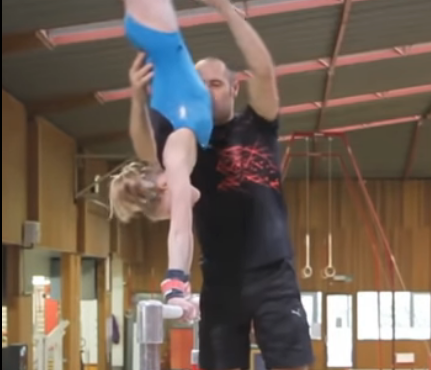
\includegraphics[width=\linewidth]{training1.png}
  \caption{Human Protective Boundary}
\end{subfigure}%
\begin{subfigure}{.25\textwidth}
  \centering
  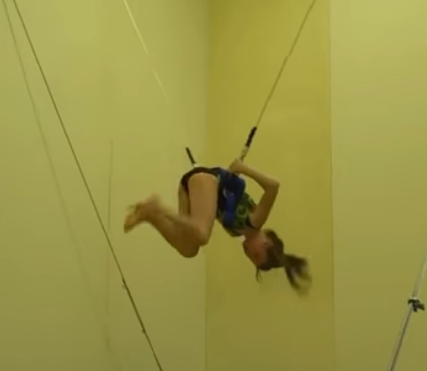
\includegraphics[width=\linewidth]{training2.png}
  \caption{Harness Protective Boundary}
\end{subfigure}
\caption{Protective Boundary in Atheletic Training}
\label{fig:athelete}
\end{figure}

We implemented the proposed protective boundary scheme on various OpenAI Gym environments as a proof of concept and we conclude that when the boundaries are set appropriately, accelerated learning can be achieved and the resulting agents have indistinguishable evaluation score compare to the agents trained with normal methods. We have confidence in our conclusion since while randomness might underline one set of data, it is highly unlikely that randomness alone can explain the same observations made in different set of experiments. 

In section I we introduce reinforcement learning in the language of control. In section II we introduce our proposed protective boundary scheme for accelerated RL agent training. In section III, we detail the results of all our experiments. While the experiments are conducted in OpenAI Gym simulated environment, we consciously designed things in a way such that it can be implemented in the physical world as well. In the final section, we conclude what we have learned from our experiments and layout directions for further research.

\section{Reinforcement Learning For Control Researchers}

\subsection{Note on Notation and Nomenclature}
The first barrier that stands between control researchers and RL is the jungle of notations. At this point, just about every researcher has his own symbolic system. As noted by Warren Powell in his 2014 introductory paper on Approximate Dynamic Programming: "Somewhat frustratingly, these communities have also developed different vocabularies and different notational systems." Yet in the same breath, Powell introduced a new set of customized notation. \cite{Powell2009WhatYS} Here, we merely try to point out the differences to make life easier for control researchers. Control communities use the notation system introduced by Lev Pontryagin. The state is denoted by $ \mathcal{X}$, conventionally a letter representing the unknown. Action is denoted by $\mathcal{U}$, the first letter of Russian for action. The dynamics and stochasticity is captured by physical model constraints $x_{t+1}=f(x_t,u_t,e_t)$ where e denotes the noise of a system. The objective is usually to minimize the cost function $\mathcal{J(.)}$. Reinforcement Learning communities adapt their notation system from the field of Operations Research. State is denoted $\mathcal{S}$, Action is denoted $\mathcal{A}$. The system dynamics and stochasticity is captured via transition matrix $\mathcal{P}$ of a Markov Decision Process. The objective of RL is the maximize the reward function $\mathcal{R(.)}$. We would like to present this note to control researchers at the beginning of our paper as they might find the reinforcement learning literature notation rather confusing.

Richard Sutton, the funding father of Reinforcement Learning, uses terminologies that can be overloaded and confusing such as Monte Carlo, Temporal Difference(TD), in his book Introduction to Reinforcement Learning \cite{Sutton1998IntroductionTR}. Although the control community also has to deal with the sequential aspect of a problem, the terminologies devised there is much more down-to-earth and straightforward, such as one-step look ahead, n-steps look ahead. In the context of RL, Monte Carlo simply means update with data collected from an entire episode. Temporal Difference means update with data collected with one step. TD($\lambda$) means update with data collected with $\lambda$ steps. Maybe one thing the control community can pick up from that of RL is how to cultivate a sense of mystique. If you can obfuscate with Latin, why illuminate with plain words? We should be grateful that Richard Sutton did not name his method Differentiali Temporum.

\subsection{From Dynamic Programming to RL}
In order to introduce RL to control researchers, we framed RL in the language of optimization, which is build on Benjamin Recht's presentation \cite{Recht2018ATO}. Broadly speaking, there are three revenues where neural network based approximation finds its way into optimization as shown in figure \ref{fig:1}.

\begin{figure}
    \centering
    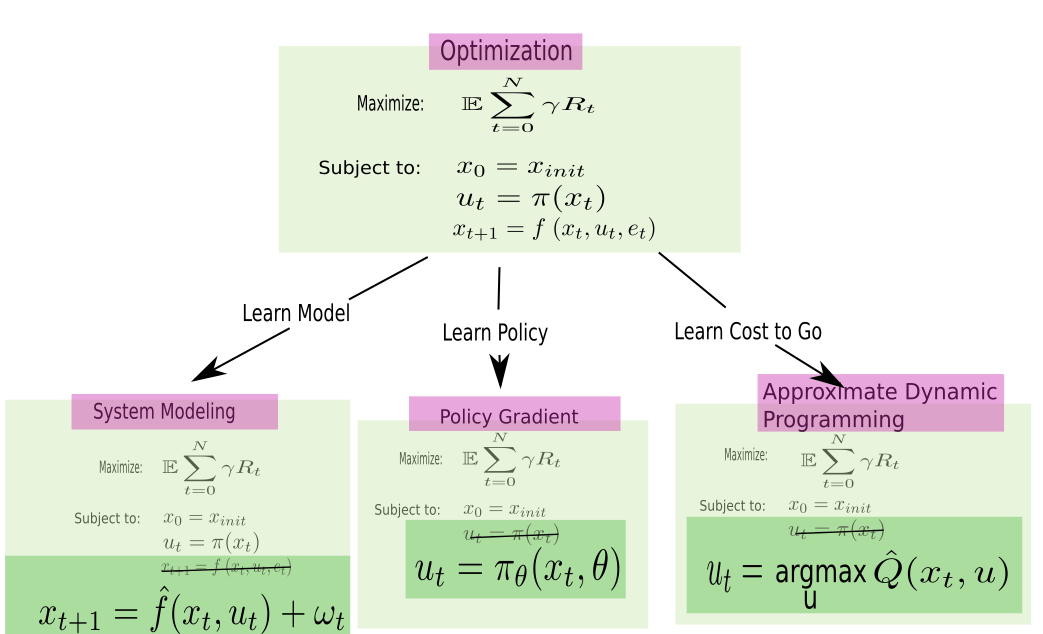
\includegraphics[width=0.5\textwidth]{Control.png}
    \caption{From Optimization to Learning}
    \label{fig:1}
\end{figure}

Reinforcement Learning is not a new subject, control researchers probably know it by the name Approximate Dynamic Programming or Neuro Dynamic Programming. When the first batch of reasonable RL results was introduced, it was met with coldness by people in control. The preface of Bertseka's book Neuro Dynamic Programming provides a good sample of how reinforcement learning is perceived by the control community back in 1996: "...These methods (Reinforcement Learning) were aiming to provide effective suboptimal solutions to complex problems of planning and sequential decision making under uncertainty, that for a long time were thought to be intractable. Our first impression was that the new methods were ambitious, overly optimistic, and lacked a firm foundation...Three years later, after a lot of study, analysis, and experimentation, we believe that our initial impressions were largely correct." \cite{Bertsekas1996NeuroDynamicP}

Today, what has changed is not the theoretical foundation of RL, which is as leaky as it was in 1996, but the computational infrastructure that undergirds it. Before 2010, the predominant tools for function approximation are kernel methods, where feature spaces are used to transform nonlinear functions into linear space such that regression can be performed. Today, the default function approximator is neural networks. Another major change in computation is that of GPU based parallelization. Before the advent of CUDA, GPU programming requires a Ph.D. in computer graphics. Today, anyone who is proficient in C/C++ can program GPU to parallelize their computation. Software packages such as PyTorch and Tensorflow made this even easier.

Dynamic Programming is simply reasoning backwards. Take trajectory optimization for instance, if we know the desired final state and system constraints then we can simply compute backwards on the penultimate step, and the computing chain flows backwards from there. The prerequisites for a successful dynamic programming based controller are two-pronged: first, the observation space and action space are reasonably small; second, the system dynamics function is known. Neither is easily met in real life scenario.

Approximate Dynamic Programming comes in when the action space and observation space are large. Instead of computing for exact one to one relationship between observation and action choice, we use a function approximator to capture all the control information. Yet even for approximate dynamic programming, the reasoning backwards requires knowing system dynamics function. RL finally provides the bridge to extend approximate dynamic program to circumstances when the system model is unknow.

In most intuitive step to incorporate unknown system dynamics into approximate dynamic programming 

Neural Networks can be used to approximate system dynamics function, which is topic for System Identification researchers. While it is true that model based reinforcement learning and offline learning has gain tractions in recent years, in this paper, we won't focus on this line of research. Neural Netoworks can also be used to approximate control policy and the cost-to-go in approximate dynamic programming. A bootstrap structure is the most critical step in extending approximate dynamic programming to cases where the system function is unknow. Cost-to-go, which is computed based on system dynamics is used in order to choose an action. In RL, the agent just guess the cost-to-go and make choices according to its guesses. As the agent accumunate data based on our guesses, it refines the process it utilizes to come up with estimations. To put this process simply: when an agent learns to control an unknown system, it made assumptions on the steps ahead and base its action on those assumptions. After observing experiments data, the agent calibrate its ability to guess.









 While out joints can have all kinds of combinatorial movement, we only use a few of those even in the most rigirous scenarios such as yoga. It seems to us that there are tools such as protective boundaries that human use to accelerate our learning. Is there a way to minimize the inefficiencies present in reinforcement learning and get closer to human level efficiency? Immitation learning seek to address this issue by provide a model trajectory, and meta-learning see to address this by provide agents with a sense of physics. 
\subsection{Combine Policy Approximation and Cost-to-go Approximation}
\subsubsection{Advantage Actor Critic(A2C)}
\subsubsection{Trust Region Actor Critic}
\subsubsection{PPO}
\subsection{Entropy Regularization}
\section{Protective Boundary}
\subsection{Protective Boundaries in Atheletic Training}
Have you ever wondered how do world class athelets such as gymnists, figure skaters, divers accomplish feats that are seemingly impossible to us ordinary human?  

\subsection{Implement Protective Boundary in OpenAI Gym}
We implemented our protective boundary experiments in OpenAI Gym as a proof of concept. We are cognicent of the fact that most of the control tasks facing our readers would be in real physical worlds. Therefore, we designed the protective barrier in a manner such that they can be swiftly adapted in real world should any researchers chooce to do so.

OpenAI Gym is a simulation environment build for reinforcement learning agents. Agent observe the state vector, reward, and termination after taking a step, which is implemented in the following sentense: observation, reward, done, info = environment.step(action).

There are various reinforcement learning agents implementations out there in the market. We choose tensorforce for this paper because it is routinely maintained, updated and with detailed instrictions on how each agent is constructed. We choose PPO agents for our experiments with entropy regularization. We set the parameters of the agents of the agents not to minimize the training steps but to accenturate the difference between our approach of training and that of normal training. Agents in the same environments share the same parameters, the only difference is weather or not they have protective boundaries.

Our experiments are conducted over the following environments: CartPole, with discrete action space; Inverted Pendulum, with continuous action space; Inverted Double Pendulum; Hopper; Walker. We did not implement our approach on more sophisiticated environments such as Humanroid and HumanroidStandup due to hardware constraints. Yet we feel that for the data we collected, our approach has shown acceleration on training when the boundaries are setup approapriately. Researchers with more powerful compute should check to see if our scheme works for environments that is harder to simulate.

One difficulty facing control researchers when they first interact with OpenAI Gym environment is the lack of documentations. We took the time to figure out what does agents observe in each environment and included the detailed notes in our code.

\subsection{CartPole and Inveretd Pendulum}
CartPole's Observation Space is: [Cart Position, Cart Velocity, Pole Angle, Pole Angular Velocity]. The discrete action space is for cartpole: [Push Cart to the left, Push cart to the right]. The continuous action space for Inverted Pendulum is an action ranging from -1 to 1, where -1 means the acturator moves the cart to the left with maximum power and 1 means the acturator moves the cart to the right with maximum power. The terminal states of cartpole is: when the absolute value of cart position is greater than 2.4 or when the absolute pole angle is greater than 12 degrees.

We proposed three protective rings anchored on the cart, at the height of middle of the pole, each allowing the pole to fall at maximum absolute value of 6,8.4,10.8 degrees respectively, as shown by the figure \ref{fig:cartpolePB}. The experiment result for cartpole suggest simimar conclusion as shown by figure \ref{fig:InvertedPendulum}.


When the pole hit the protective boundary, it would push the cart back to the center, implemented by an automatic action choice of 0 or 1 depending on the sign of angle. A penulty is incurred every time the pole makes contact with the protective boundary, the penulties are set to be 0,-5,-7,-10,-12,-15 for each protective boundary. Our experiment result on cartpole are shown by figure \ref{fig:CartPole}. As the data suggest, when the boundary is set at 6 degree, it seems to be too restrictive for agent training. The best ressults is seen when the boundary is set at 10.8 degree, giving the agent plenty of rooms to adjust itself and acquiring the skill. The accelerated learning seems to be brought about mostly by the protective boundary itself instead of the penulty terms since our data suggest that when the boundary is set at the right place, all the penulties accelerate learning to a certain extend.

After the agents are done training, we also evaluate their performance on environments without protective boundaries. Our data suggest that when acceleration is achieved, the agents perform identially to the agents trained in normal enviroment.

\begin{figure}
     \centering
      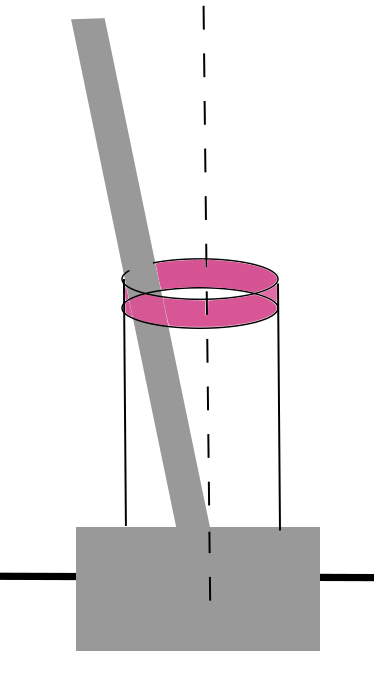
\includegraphics[width=0.1\textwidth]{cartpole1.png}
      \caption{CartPole Protective Boundary}
      \label{fig:cartpolePB}
\end{figure}

\begin{figure}
    \centering
    \captionsetup[subfigure]{font=scriptsize,labelfont=scriptsize}
    \begin{subfigure}[b]{0.5\textwidth}
      \centering
      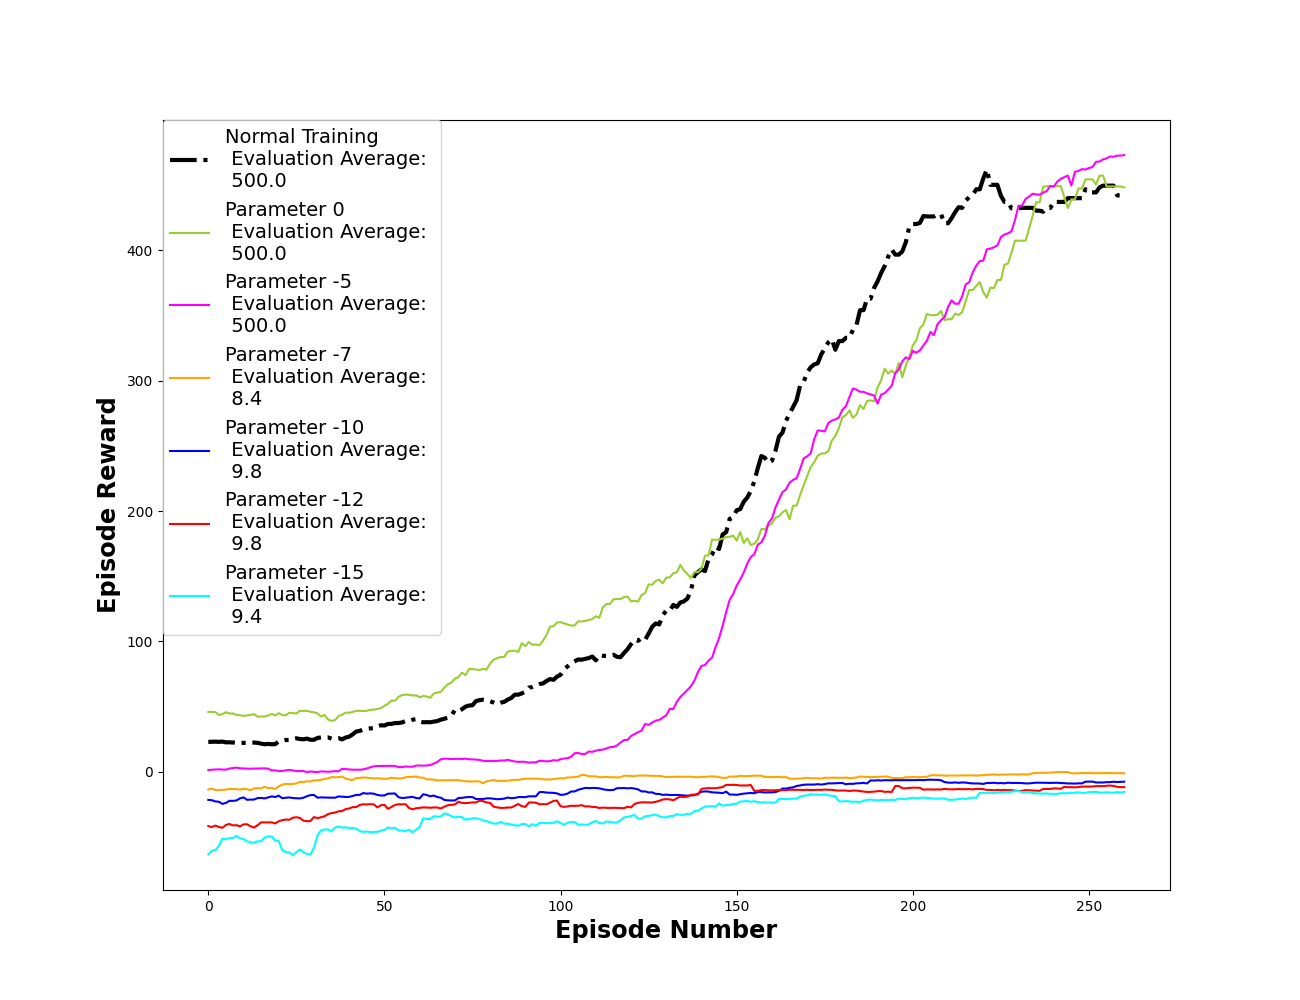
\includegraphics[width=\textwidth]{Cartpole_with_Boundary_at_0.5.png}
    \end{subfigure}
    \vspace*{0.0mm}
    \begin{subfigure}[b]{0.5\textwidth}
      \centering
      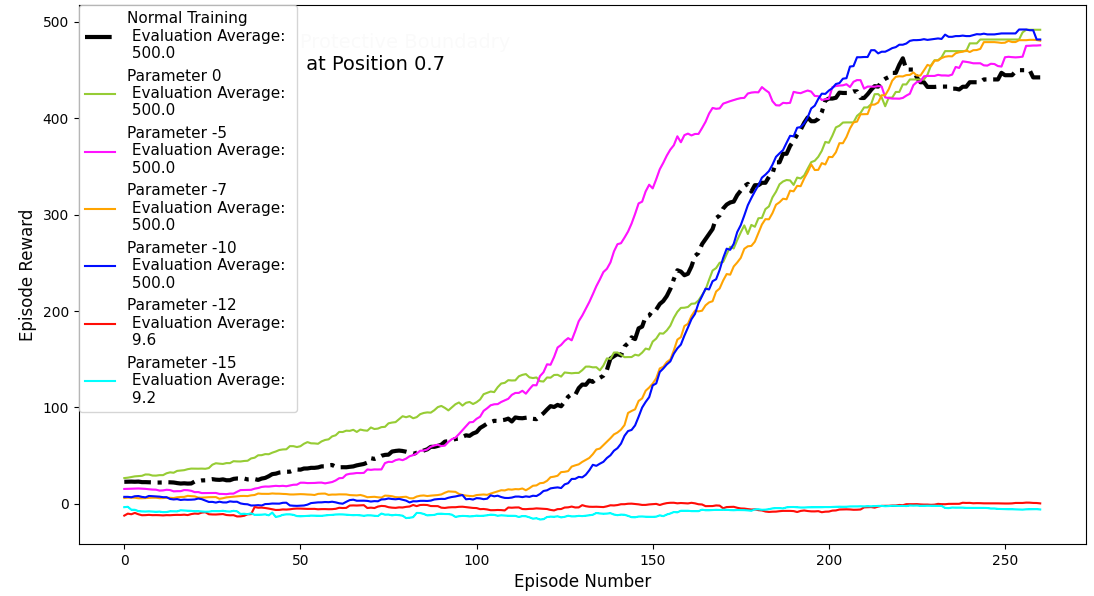
\includegraphics[width=\textwidth]{Cartpole_with_Boundary_at_0.7.png}
    \end{subfigure}
    \vspace*{0.0mm}
    \begin{subfigure}[b]{0.5\textwidth}
      \centering
      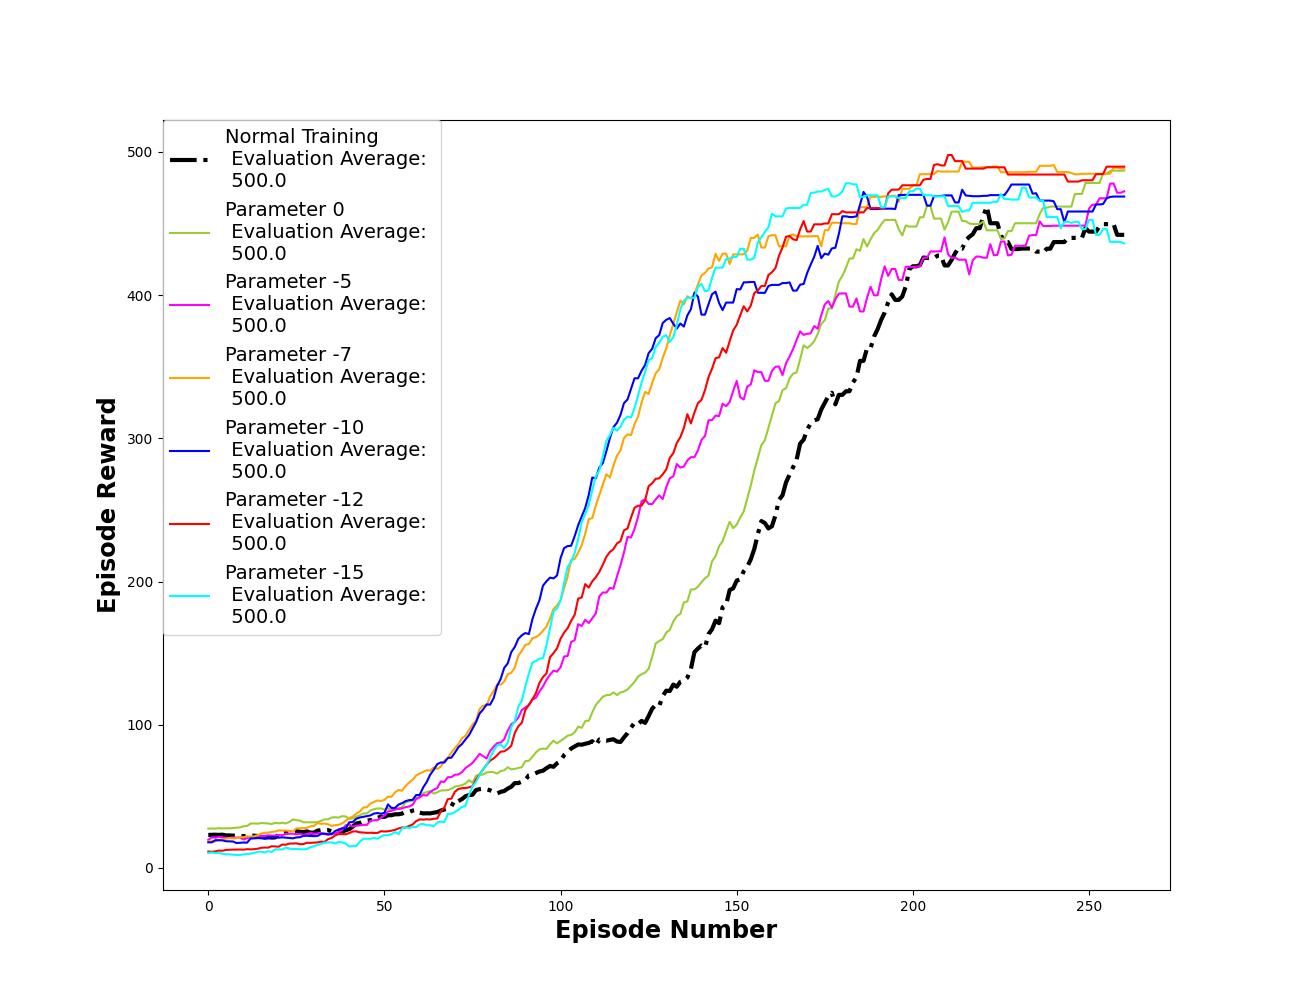
\includegraphics[width=\textwidth]{Cartpole_with_Boundary_at_0.9.png}
    \end{subfigure}
    \caption{CartPole Experiments}
    \label{fig:CartPole}
\end{figure}

\begin{figure}
    \centering
    \begin{subfigure}[b]{0.5\textwidth}
      \centering
      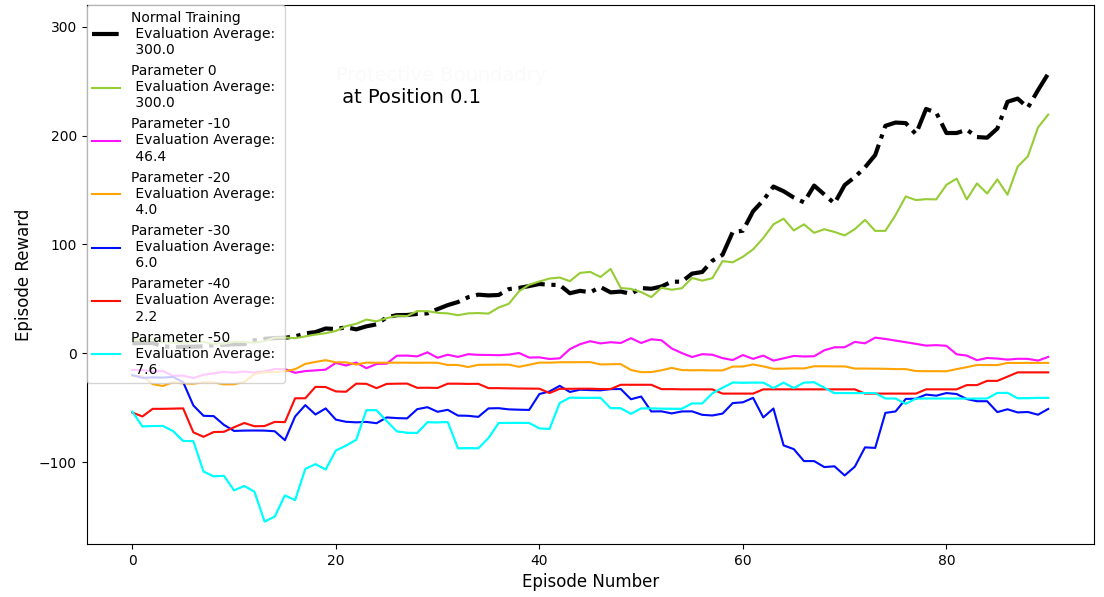
\includegraphics[width=\textwidth]{Inverted_Pendulum_with_Boundary_at_0.1.png}
    \end{subfigure}
    \vspace*{0.0mm}
    \begin{subfigure}[b]{0.5\textwidth}
      \centering
      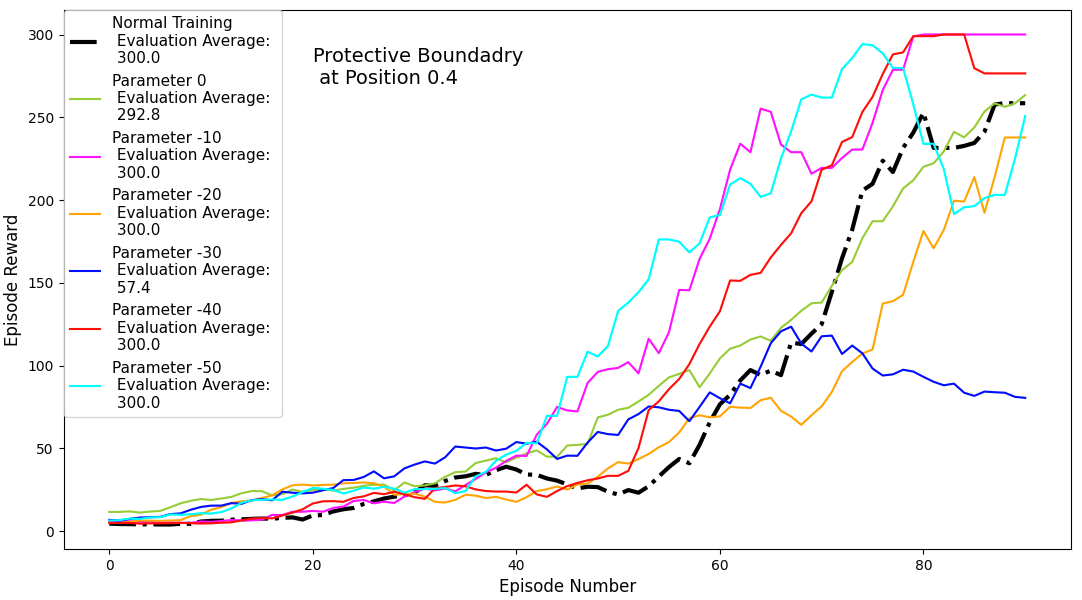
\includegraphics[width=\textwidth]{Inverted_Pendulum_with_Boundary_at_0.4.png}
    \end{subfigure}
    \vspace*{0.0mm}
    \begin{subfigure}[b]{0.5\textwidth}
      \centering
      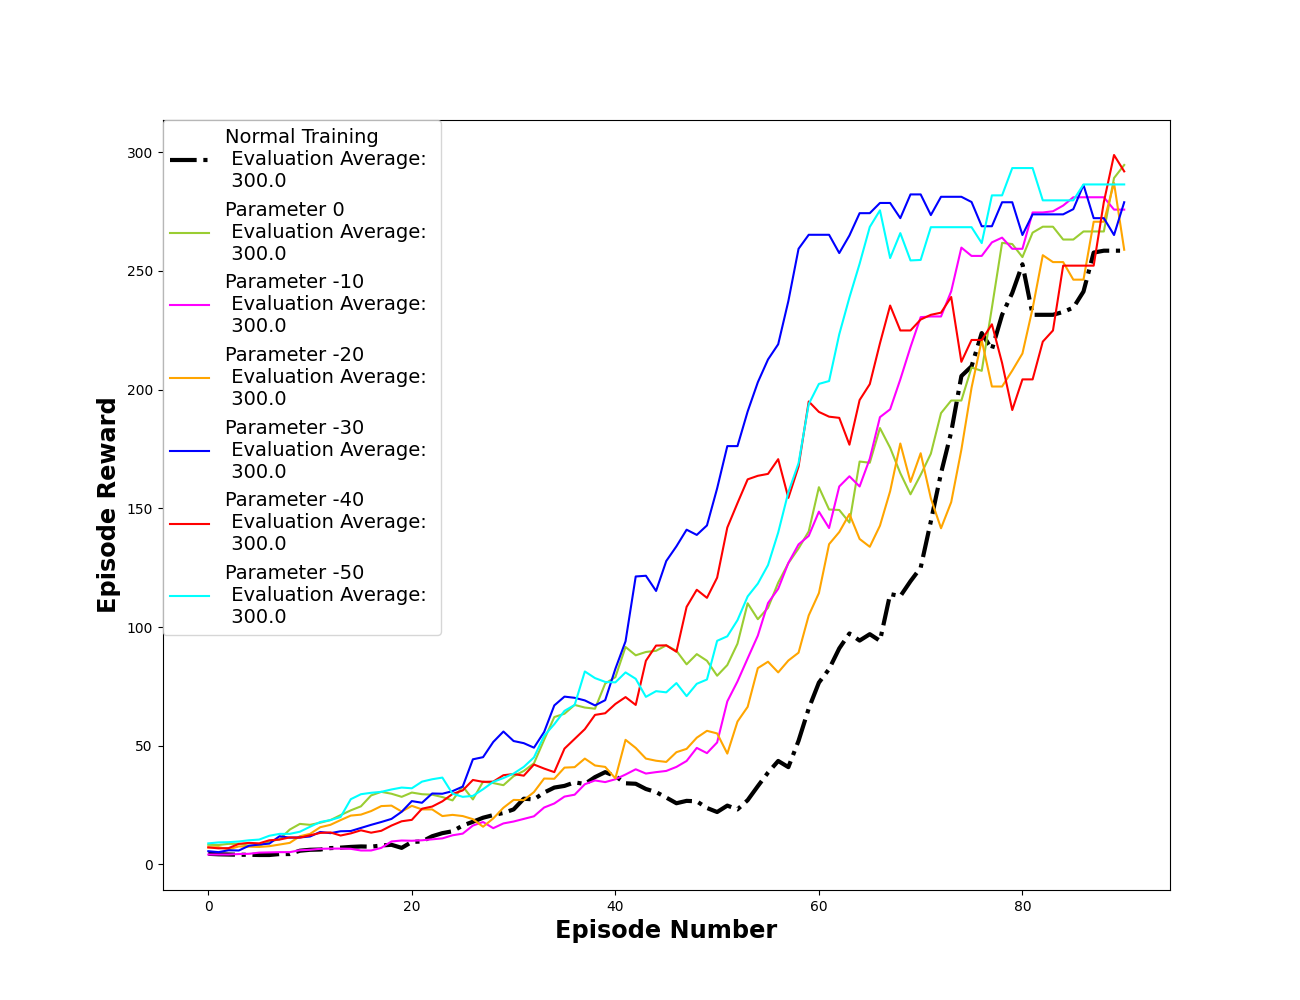
\includegraphics[width=\textwidth]{Inverted_Pendulum_with_Boundary_at_0.5.png}
    \end{subfigure}
    \caption{Inverted Pendulum Experiments}
    \label{fig:InvertedPendulum}
\end{figure}

\subsection{Inverted Double Pendulum}
The inveretd double pendulum has observation space as follows: [x position of the cart, sin($\theta_1$), sin($\theta_2$),cos($\theta_1$),cos($\theta_2$),velocity of x, angular velocity of $\theta_1$, angular velocity of $\theta_2$, constraint force on x, constraint force on $\theta_1$, constraint force on $\theta_2$]. $\theta_1$ and $\theta_2$ are the angles of the upper and lower pole perspectively.

The action space for Inverted Double Pendulum is an action ranging from -1 to 1, where -1 means the acturator moves the cart to the left with maximum power and 1 means the acturator moves the cart to the right with maximum power.

The Terminal state of double inveretd pendulum is when the y postion of the upper pole, which can not be observed by the agent falls below 1.

We design the protective boundary to be located at the same height as does the joint between upper and lower pole, as indicated by figure \ref{fig:doublePB}. The boundary allows the joint to flex for 0.4, 0.5 and 0.6 radians perepectively, each with the penulty parameters of a choice between 0,-3,-4,-5,-6,-7. When the joint extend to touch the protective boundary, an action of -1 or 1 would be automatically applied to rectify the situation, depending on the sigh of the angles.

\begin{figure}
     \centering
      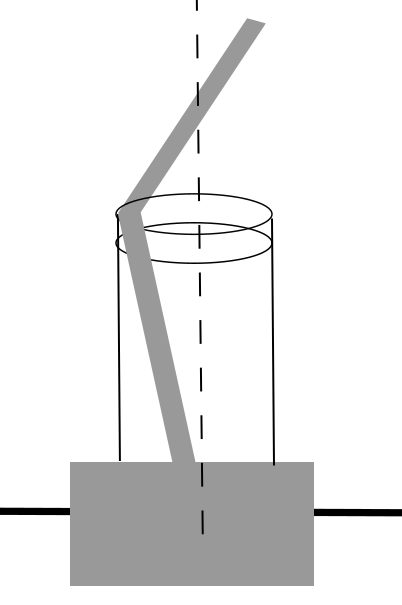
\includegraphics[width=0.1\textwidth]{cartpole2.png}
      \caption{Inveretd Double Pendulum Protective Boundary}
      \label{fig:doublePB}
\end{figure}

Our experiments result is show by figure \ref{fig:Double Pendulum} with conclusion similar to that of cartpole and inverted pendulum results. When the protective boundary is set at 0.4 radius, it hinders learning rather than facilitate it. When the boundary is set at 0.5 radius with a penulty parameter of -7, we see the most drastic acceleration of agent training. However, when the boundary is set at 0.6 radius, it seems to have given the agent too much flexibility since the result suggest that the acceleration is not as profound compare to that of boundary set at 0.5.

\begin{figure}
    \centering
    \begin{subfigure}[b]{0.5\textwidth}
      \centering
      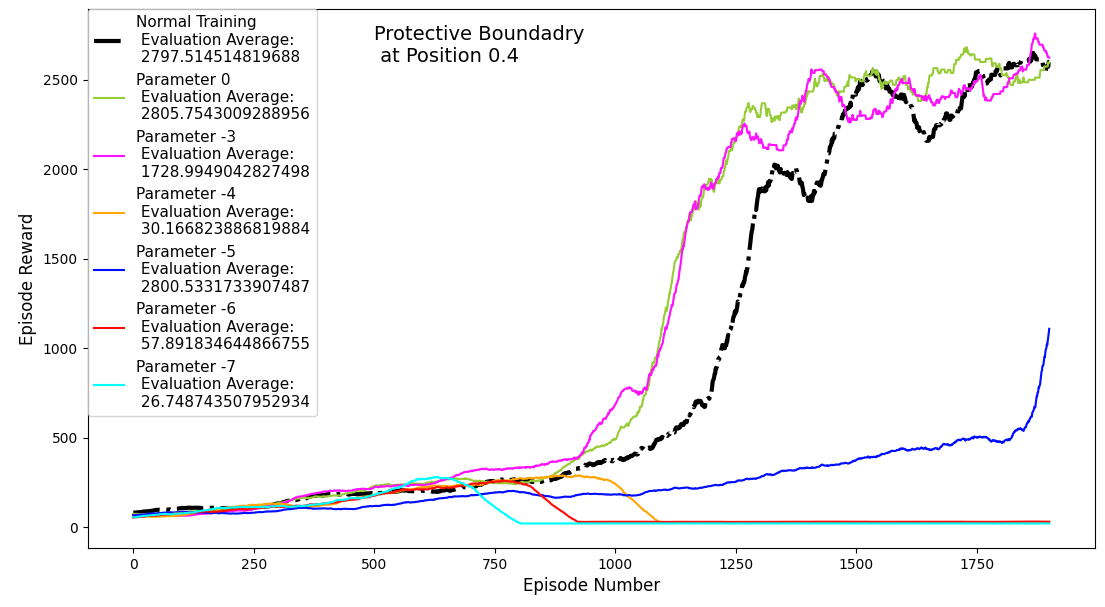
\includegraphics[width=\textwidth]{Double_Pendulum_with_Boundary_at_0.4.png}
    \end{subfigure}
    \vspace*{0.0mm}
    \begin{subfigure}[b]{0.5\textwidth}
      \centering
      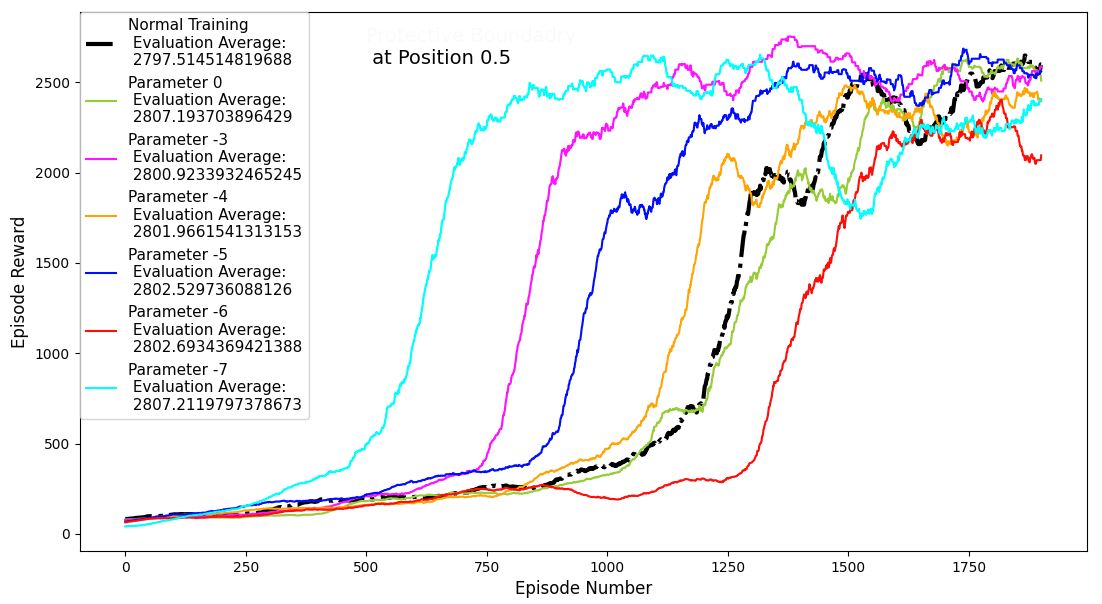
\includegraphics[width=\textwidth]{Double_Pendulum_with_Boundary_at_0.5.png}
    \end{subfigure}
    \vspace*{0.0mm}
    \begin{subfigure}[b]{0.5\textwidth}
      \centering
      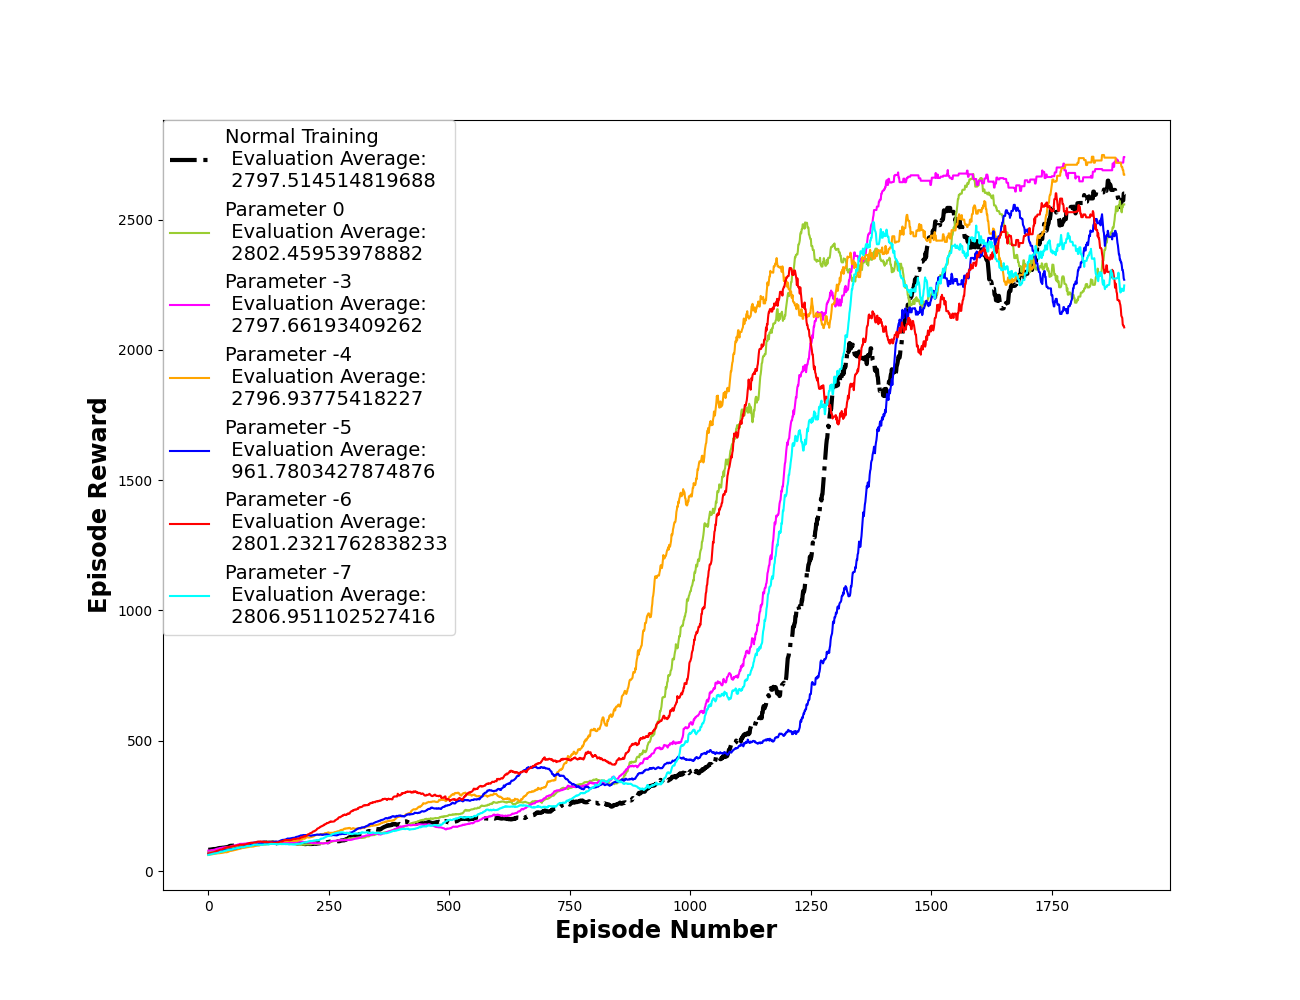
\includegraphics[width=\textwidth]{Double_Pendulum_with_Boundary_at_0.6.png}
    \end{subfigure}
    \caption{Inverted Double Pendulum Experiments}
    \label{fig:Double Pendulum}
\end{figure}


\subsection{Hopper}
The observation space of hopper is the following: [z position, y position, thigh joint angle, leg joint angle, foot joint angle, velocity at x axis, velocity at z axis, velocity at y axis, angular velocity of thigh joint, angular velocity of leg joint, angular velocity of foot joint].

The action space of hopper are three continuous action choices for three acturators [thigh acturator, leg acturator, foot acturator]. The range of for acturators are -1, which means apply force towards the negative direction with maximum power, and 1 which means apply force towards the positive direction with maximum power.

The terminal states for hopper are when the absolute y position is greater than 0.2.

The protective boundary is set with the y position at 0.05, 0.1 and 0.15, each with the penulty parameters that is chosen from 0,-3,-5,-7,-10 as shown by figure \ref{fig:hopperPB} When the agent touches the protective boundary, we gentenly guide it slightly towards the smaller y position, and the velocities terms are all set to zero in this step. We seek to mimic how a coach would guide an atheletes towards the desired trajectory during training. When the athelete is about to fall, the coach would take over and apply the apppriate force such that the trajectory of that athelete is reset slightly and he or she get to experience more with states that are pertinent to his/her training.

Our experiment result is show by fiture \ref{fig:Hopper}. Similar to the conclusion drawn with previous experiments on cartpole, inverted pendulum and inverted double pendulum, when the protective boundary is set too narrowly at 0.05 y position, it restrict the agent and almost completely halt the agent training. The best training accepration is observed when the boundary is set at 0.15 y position, irrestpect of the penulty parameter.

\begin{figure}
     \centering
      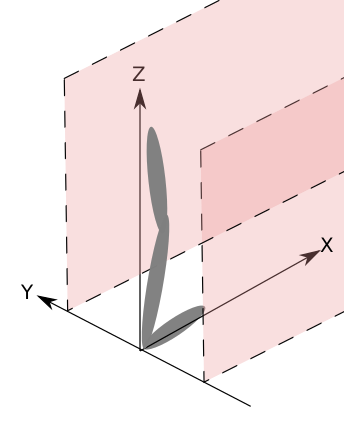
\includegraphics[width=0.2\textwidth]{hopper.png}
      \caption{Hopper Protective Boundary}
      \label{fig:hopperPB}
\end{figure}

\begin{figure}
    \centering
    \begin{subfigure}[b]{0.5\textwidth}
      \centering
      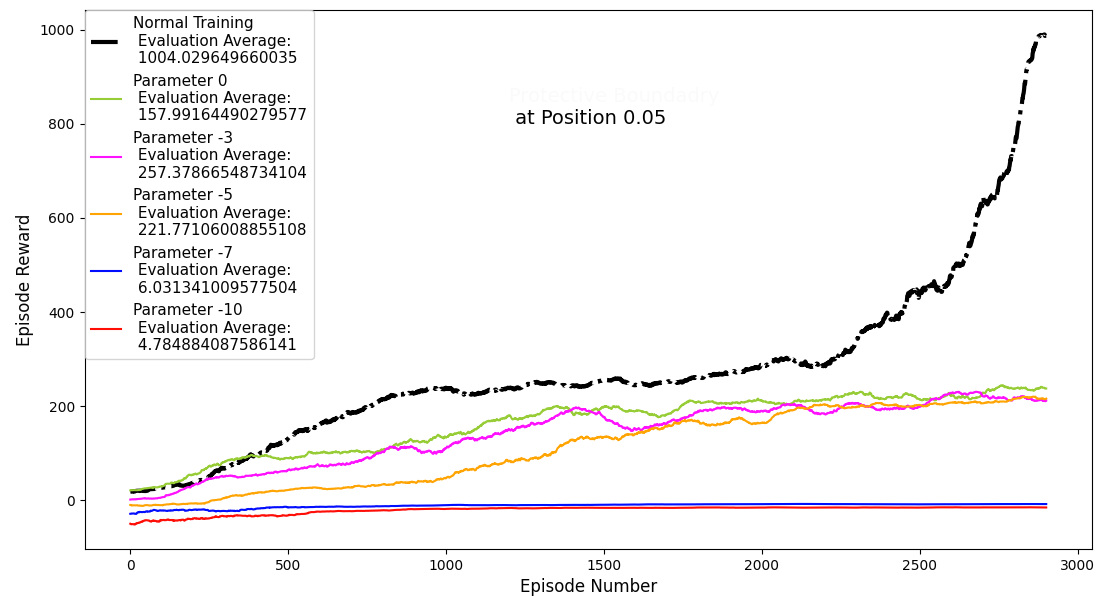
\includegraphics[width=\textwidth]{Hopper_with_Boundary_at_0.05.png}
    \end{subfigure}
    \vspace*{0.0mm}
    \begin{subfigure}[b]{0.5\textwidth}
      \centering
      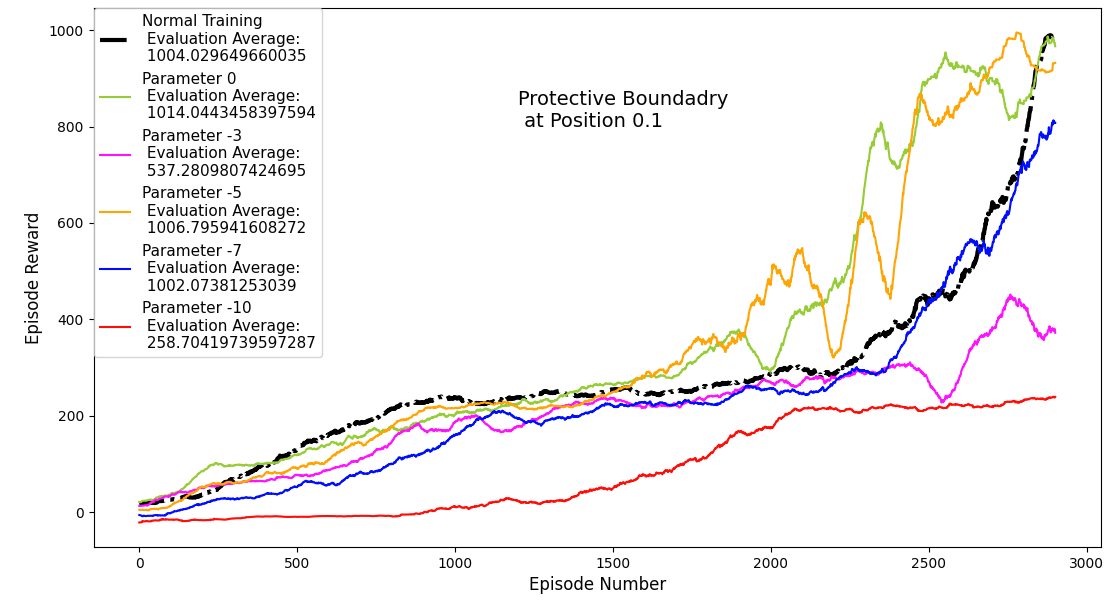
\includegraphics[width=\textwidth]{Hopper_with_Boundary_at_0.1.png}
    \end{subfigure}
    \vspace*{0.0mm}
    \begin{subfigure}[b]{0.5\textwidth}
      \centering
      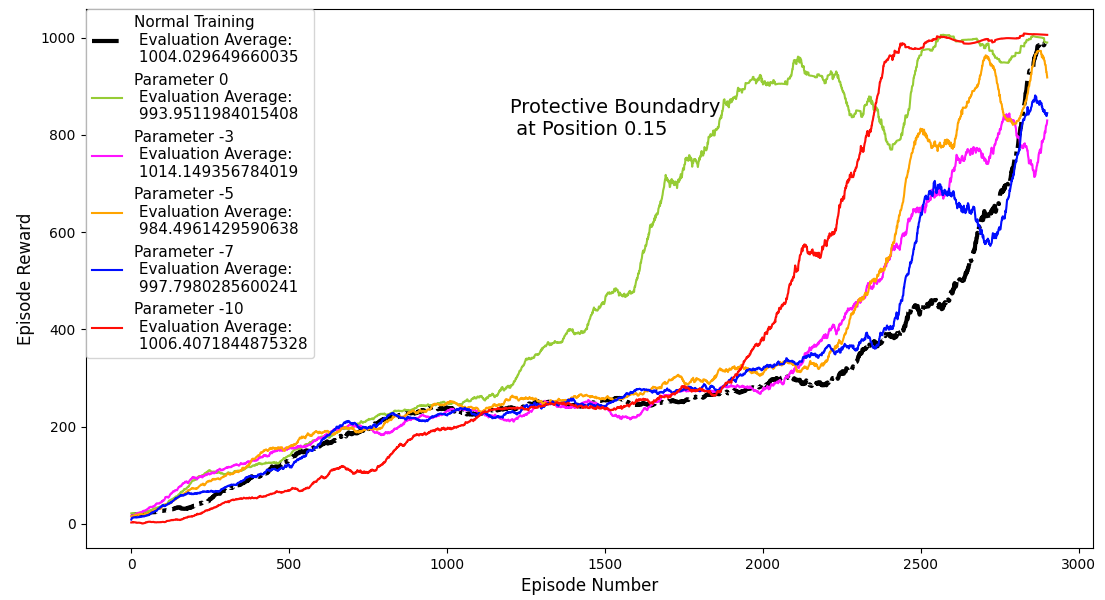
\includegraphics[width=\textwidth]{Hopper_with_Boundary_at_0.15.png}
    \end{subfigure}
    \caption{Hopper}
    \label{fig:Hopper}
\end{figure}


\subsection{Walker2d}
The walker environment's observation spaces are as the following: [z positoin, y position, right thigh joint angle, right leg joint angle, right foot joint angle, left thigh joint angle, left leg joint angle, left foot joint angle, velocity along x axis, velocity along z axis, velocity along y axix, angular velocity for right thigh joint, angular velocity for right leg joint, angular velocity for right foot joint, angular velocity for left thigh joint, angular velocity for left leg joint, angular velocity for left foot joint]

There are 6 acturators for right thigh joint, right leg joint, right foot joint and left thigh joint, left leg joint, left foot joint perspectively. The range for the motors are -1 which means apply force towards the negative direction with maximum power and 1 which means apply force towards the positive direction with maximum power.

The terminal states are when the z position falls below 0.8 or raise above 2 or the absolute value of y position is greater than 1.

The protective boundary is set with the y position at 0.3, 0.7 and 0.9, each with the penulty parameters that is chosen from 0,-5,-10,-15,-20 as shown by figure \ref{fig:walkerPB}. Similar to the protective boundary of hopper, when the agent touches the protective boundary in walker environment, we gentenly guide it slightly towards the smaller y position, and the velocities terms are all set to zero in the mean time.

Our experiment result is show by fiture \ref{fig:Walker}. Yet again the experiment result suggest the same conclusion: when the boundary is positioned at 0.1, it acts as a barrier to training.

\begin{figure}
     \centering
      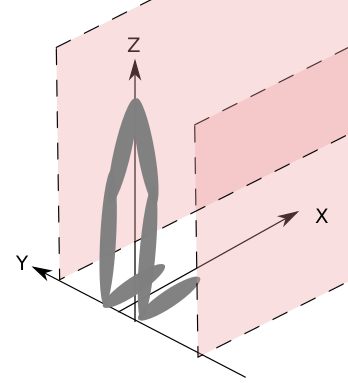
\includegraphics[width=0.2\textwidth]{walker.png}
      \caption{Walker2d Protective Boundary}
      \label{fig:walkerPB}
\end{figure}

\begin{figure}
    \centering
    \begin{subfigure}[b]{0.5\textwidth}
      \centering
      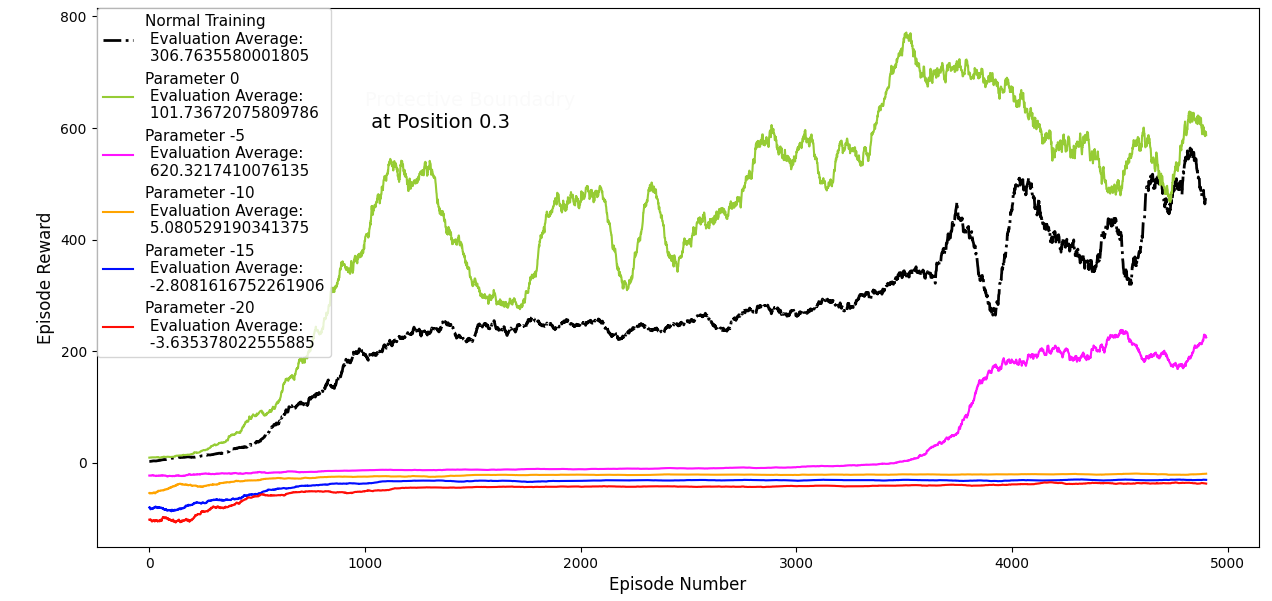
\includegraphics[width=\textwidth]{Walker_with_Boundary_at_0.3.png}
    \end{subfigure}
    \vspace*{0.0mm}
    \begin{subfigure}[b]{0.5\textwidth}
      \centering
      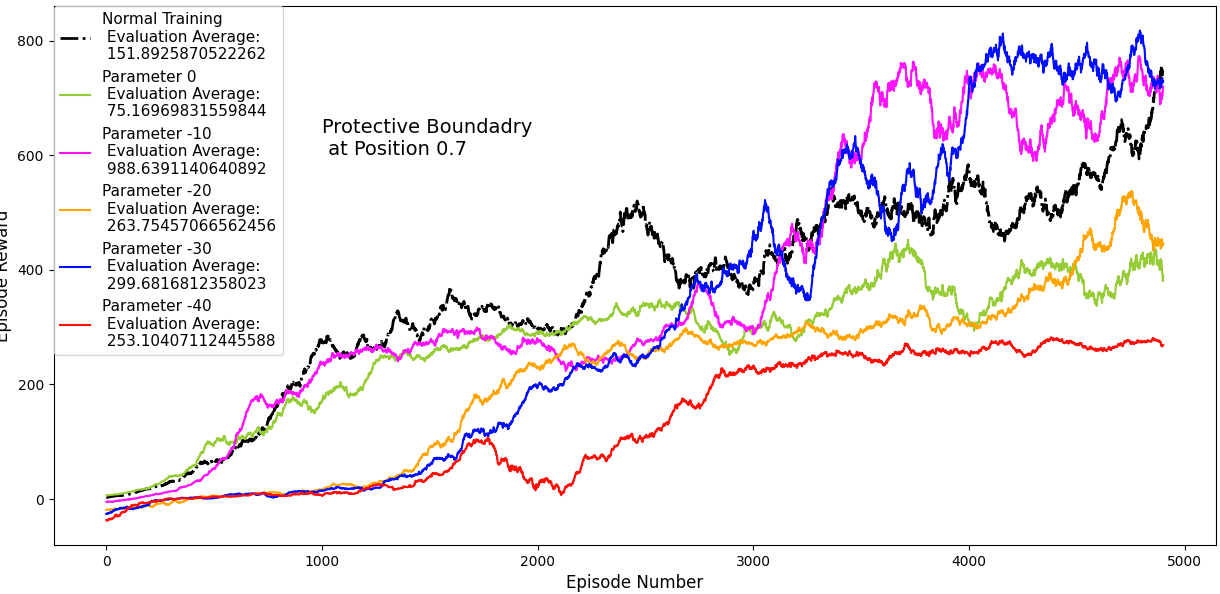
\includegraphics[width=\textwidth]{Walker_with_Boundary_at_0.7.png}
    \end{subfigure}
    \vspace*{0.0mm}
    \begin{subfigure}[b]{0.5\textwidth}
      \centering
      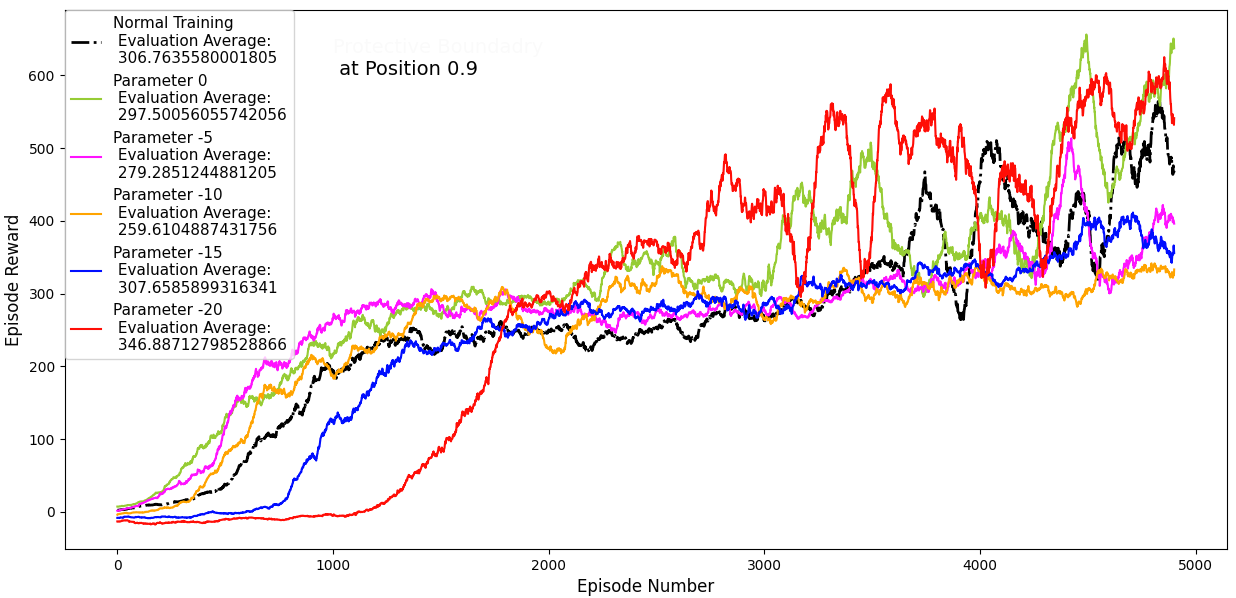
\includegraphics[width=\textwidth]{Walker_with_Boundary_at_0.9.png}
    \end{subfigure}
    \caption{Walker2D}
    \label{fig:Walker}
\end{figure}

\subsection{HalfCheetah}
The walker environment's observation spaces are as the following: [z positoin, y position, right thigh joint angle, right leg joint angle, right foot joint angle, left thigh joint angle, left leg joint angle, left foot joint angle, velocity along x axis, velocity along z axis, velocity along y axix, angular velocity for right thigh joint, angular velocity for right leg joint, angular velocity for right foot joint, angular velocity for left thigh joint, angular velocity for left leg joint, angular velocity for left foot joint]

There are 6 acturators for right thigh joint, right leg joint, right foot joint and left thigh joint, left leg joint, left foot joint perspectively. The range for the motors are -1 which means apply force towards the negative direction with maximum power and 1 which means apply force towards the positive direction with maximum power.

The terminal states are when the z position falls below 0.8 or raise above 2 or the absolute value of y position is greater than 1.

The protective boundary is set with the y position at 0.3, 0.7 and 0.9, each with the penulty parameters that is chosen from 0,-5,-10,-15,-20 as shown by figure \ref{fig:cheetahPB}. Similar to the protective boundary of hopper, when the agent touches the protective boundary in walker environment, we gentenly guide it slightly towards the smaller y position, and the velocities terms are all set to zero in the mean time.

Our experiment result is show by fiture \ref{fig:Cheetah}. Yet again the experiment result suggest the same conclusion: when the boundary is positioned at 0.1, it acts as a barrier to training.

\begin{figure}
     \centering
      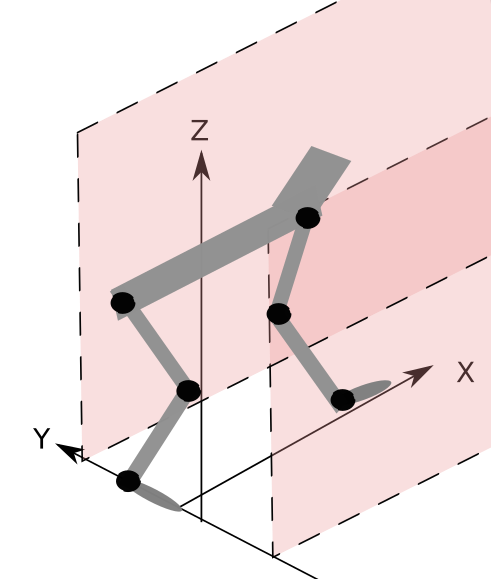
\includegraphics[width=0.2\textwidth]{cheetah.png}
      \caption{HalfCheetah Protective Boundary}
      \label{fig:cheetahPB}
\end{figure}

\begin{figure}
    \centering
    \begin{subfigure}[b]{0.5\textwidth}
      \centering
      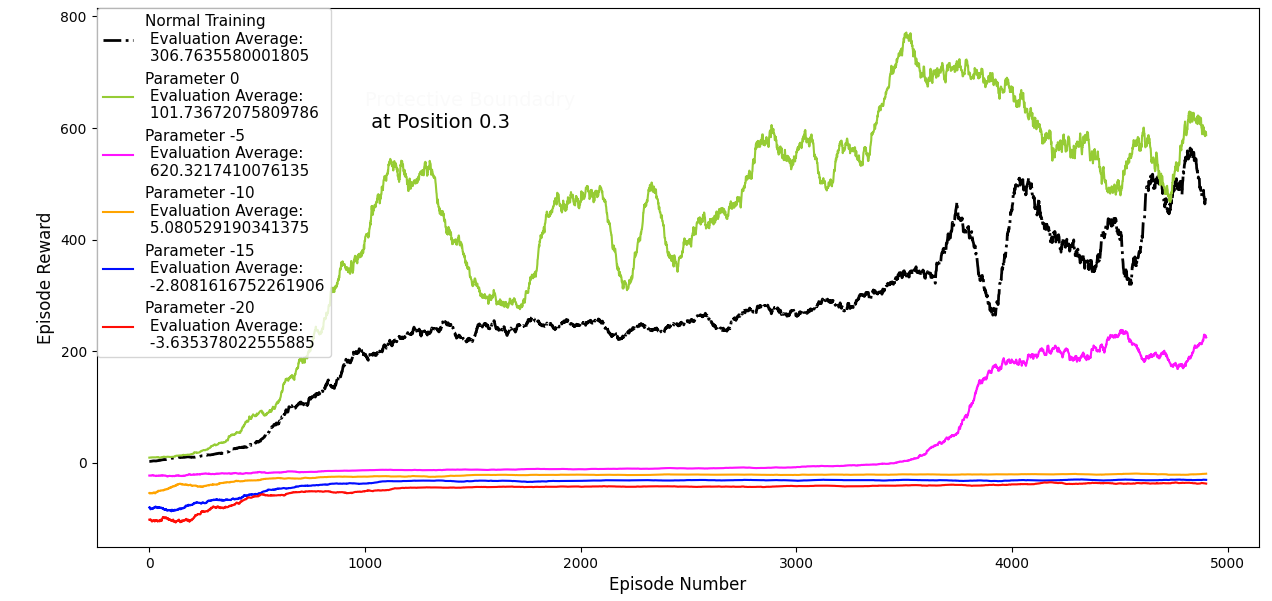
\includegraphics[width=\textwidth]{Walker_with_Boundary_at_0.3.png}
    \end{subfigure}
    \vspace*{0.0mm}
    \begin{subfigure}[b]{0.5\textwidth}
      \centering
      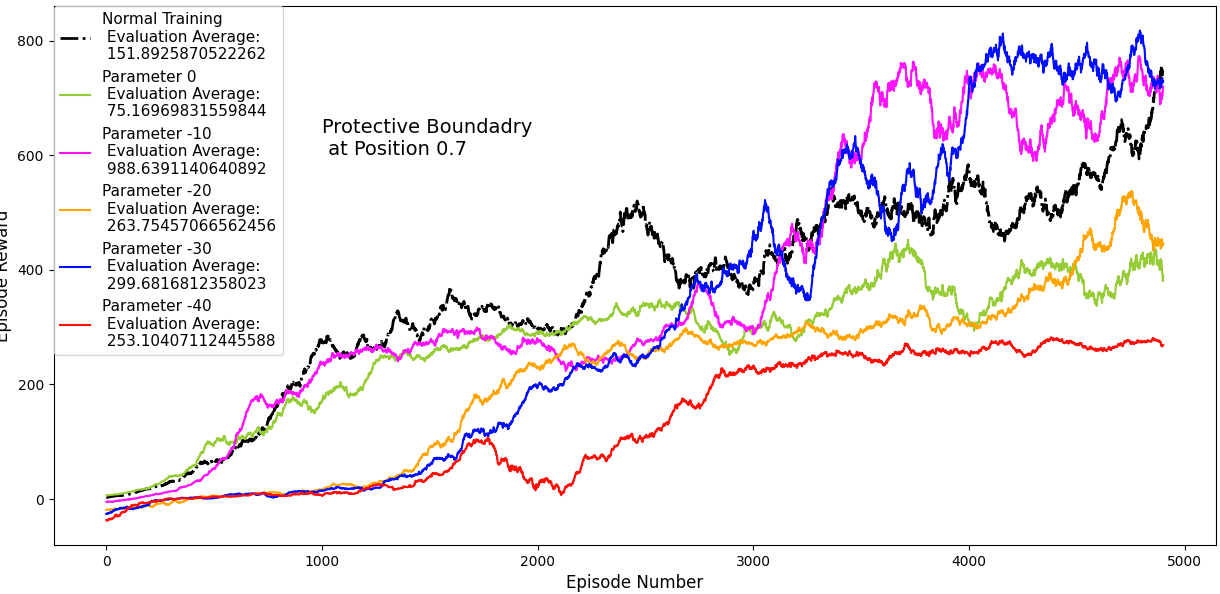
\includegraphics[width=\textwidth]{Walker_with_Boundary_at_0.7.png}
    \end{subfigure}
    \vspace*{0.0mm}
    \begin{subfigure}[b]{0.5\textwidth}
      \centering
      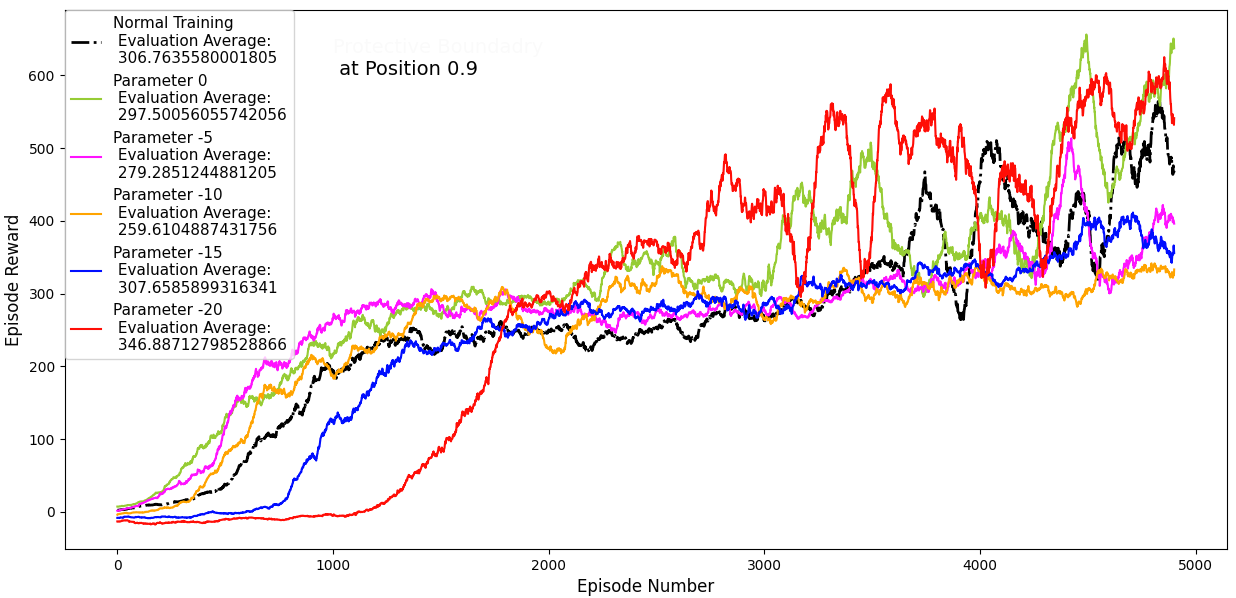
\includegraphics[width=\textwidth]{Walker_with_Boundary_at_0.9.png}
    \end{subfigure}
    \caption{HalfCheetah}
    \label{fig:Cheetah}
\end{figure}
\section{Conclution}
As shown by our experiments, when the position and punishing parameter of protective boundary is appropriate, reinforcement learning agent training can be greatly accelerated, much like human atheletes accelerate their acquistion of skills with protective equipments. We have only done experiments on the ones require lower computational power as a proof of concept and we encourage readers of our paper with access to more compute to apply to our idea to enviroments such as humanroid and humanroid standup.

 Our proof of concept data seems to suggeset that when the boundary is set too restrictively, it hinders rather than facilitate learning. Overall, the position of the boundary is more critical compare to penulty parameter, however when the penulty parameter is set too harshly, the learning process can be slowed. The rule of thumb we used during our experiments is that the punishing parameter should be roughly the same as the reward, but with negative sign.

 The evaluation result of agents trained with protective boundaries also suggest that when the boundary is set correctly, the agent can perform as well as does the agents trained in normal environment.

 Our result, albeit just proof of concept at this point should be exciting news for those who are interested in applying reinforcement learning to real world scenarios. Acceleration is possible, if we research more into how to set up the protective boundaries.In our experiments, position and penulty parameter of protective boundary is set in a haphazard fashion. Analytical frameworks is required in order to solve this in a systematic manner.

 We are reaching out to vairous researchers to further this line of research, and we look forward to welcoming more researchers to join us.

\bibliographystyle{IEEEtran}
\bibliography{Bibliography}
%\printbibliography



\end{document}
